\documentclass[a4paper]{beamer}

\usepackage[english]{babel}
\usepackage[utf8]{inputenc}
\usepackage[T1]{fontenc}
\usepackage{listings}

\usepackage{../thesis/sty/pgf-umlsd}

\usepackage{tikz}
\usetikzlibrary{positioning,shapes,arrows,chains,decorations.pathreplacing}

\lstset{
    numbers=left
}

% Template for talks using the Corporate Design of the Freie Universitaet
%   Berlin, created following the guidelines on www.fu-berlin.de/cd by
%   Tobias G. Pfeiffer, <tobias.pfeiffer@math.fu-berlin.de>
% This file can be redistributed and/or modified in any way you like.
%   If you feel you have done significant improvements to this template,
%   please consider providing your modified version to
%   https://www.mi.fu-berlin.de/w/Mi/BeamerTemplateCorporateDesign

\usepackage{amsmath,listings}

%%% FU logo
% small version for upper right corner of normal pages
\pgfdeclareimage[height=0.9cm]{university-logo}{resources/fu-logo}
\logo{\pgfuseimage{university-logo}}
% large version for upper right corner of title page
\pgfdeclareimage[height=1.085cm]{big-university-logo}{resources/fu-logo}
%%% end FU logo

\beamertemplatenavigationsymbolsempty

% NOTE: 1cm = 0.393 in = 28.346 pt;    1 pt = 1/72 in = 0.0352 cm
\setbeamersize{text margin right=3.5mm, text margin left=7.5mm}  % text margin

% colors to be used
\definecolor{text-grey}{rgb}{0.45, 0.45, 0.45} % grey text on white background
\definecolor{bg-grey}{rgb}{0.66, 0.65, 0.60} % grey background (for white text)
\definecolor{fu-blue}{RGB}{0, 51, 102} % blue text
\definecolor{fu-green}{RGB}{153, 204, 0} % green text
\definecolor{fu-red}{RGB}{204, 0, 0} % red text (used by \alert)

% switch off the sidebars
% TODO: loading \useoutertheme{sidebar} (which is maybe wanted) also inserts
%   a sidebar on title page (unwanted), also indents the page title (unwanted?),
%   and duplicates the navigation symbols (unwanted)
\setbeamersize{sidebar width left=0cm, sidebar width right=0mm}
\setbeamertemplate{sidebar right}{}
\setbeamertemplate{sidebar left}{}
%    XOR
% \useoutertheme{sidebar}

% frame title
% is truncated before logo and splits on two lines
% if neccessary (or manually using \\)
\setbeamertemplate{frametitle}{%
    \vskip-30pt \color{text-grey}\large%
    \begin{minipage}[b][23pt]{80.5mm}%
    \flushleft\insertframetitle%
    \end{minipage}%
}

%%% title page
% TODO: get rid of the navigation symbols on the title page.
%   actually, \frame[plain] *should* remove them...
\setbeamertemplate{title page}{
% upper right: FU logo
\vskip2pt\hfill\pgfuseimage{big-university-logo} \\
\vskip6pt\hskip3pt
% title image of the presentation
\begin{minipage}{11.6cm}
\hspace{-1mm}\inserttitlegraphic
\end{minipage}

% set the title and the author
\vskip14pt
\parbox[top][1.35cm][c]{11cm}{\color{text-grey}\inserttitle \\ \small \insertsubtitle}
\vskip11pt
\parbox[top][1.35cm][c]{11cm}{\small \insertauthor \\ \insertinstitute \\[3mm] \insertdate}
}
%%% end title page

%%% colors
\usecolortheme{lily}
\setbeamercolor*{normal text}{fg=black,bg=white}
\setbeamercolor*{alerted text}{fg=fu-red}
\setbeamercolor*{example text}{fg=fu-green}
\setbeamercolor*{structure}{fg=fu-blue}

\setbeamercolor*{block title}{fg=white,bg=black!50}
\setbeamercolor*{block title alerted}{fg=white,bg=black!50}
\setbeamercolor*{block title example}{fg=white,bg=black!50}

\setbeamercolor*{block body}{bg=black!10}
\setbeamercolor*{block body alerted}{bg=black!10}
\setbeamercolor*{block body example}{bg=black!10}

\setbeamercolor{bibliography entry author}{fg=fu-blue}
% TODO: this doesn't work at all:
\setbeamercolor{bibliography entry journal}{fg=text-grey}

\setbeamercolor{item}{fg=fu-blue}
\setbeamercolor{navigation symbols}{fg=text-grey,bg=bg-grey}
%%% end colors

%%% headline
\setbeamertemplate{headline}{
\vskip4pt\hfill\insertlogo\hspace{3.5mm} % logo on the right

\vskip6pt\color{fu-blue}\rule{\textwidth}{0.4pt} % horizontal line
}
%%% end headline

%%% footline
\newcommand{\footlinetext}{\insertshortinstitute, \insertshorttitle, \insertshortdate}
\setbeamertemplate{footline}{
\vskip5pt\color{fu-blue}\rule{\textwidth}{0.4pt}\\ % horizontal line
\vskip2pt
\makebox[123mm]{\hspace{7.5mm}
\color{fu-blue}\footlinetext
\hfill \raisebox{-1pt}{\usebeamertemplate***{navigation symbols}}
\hfill \insertframenumber}
\vskip4pt
}
%%% end footline

%%% settings for listings package
\lstset{extendedchars=true, showstringspaces=false, basicstyle=\footnotesize\sffamily, tabsize=2, breaklines=true, breakindent=10pt, frame=l, columns=fullflexible}
\lstset{language=Java} % this sets the syntax highlighting
\lstset{mathescape=true} % this switches on $...$ substitution in code
% enables UTF-8 in source code:
\lstset{literate={ä}{{\"a}}1 {ö}{{\"o}}1 {ü}{{\"u}}1 {Ä}{{\"A}}1 {Ö}{{\"O}}1 {Ü}{{\"U}}1 {ß}{\ss}1}
%%% end listings


\author{Patrick Steinhardt}
\title{A Protocol for Connecting Networked Resources}
\institute{Freie Universität Berlin}

\begin{document}

\begin{frame}[plain]
    \maketitle
\end{frame}

\begin{frame}{Motivation}
    Provide a solution for connecting services with each other  guaranteeing
    \begin{itemize}
        \item confidentiality of sent data
        \item authenticity of partaking parties
        \item generality of possible services
    \end{itemize}
\end{frame}

\begin{frame}{Architecture - Entities}
    Three kind of entities are taking part in the protocol:

    \begin{description}
        \item[Server]
            \begin{itemize}
                \item hosts different services
                \item responsible for answering service discovery
                \item owns a long term signature key
            \end{itemize}
        \item[Service]
            \begin{itemize}
                \item hosted on a server
                \item handles a service-specific protocol
            \end{itemize}
        \item[Client]
            \begin{itemize}
                \item user of one or multiple services
                \item owns a long term signature key
            \end{itemize}
    \end{description}
\end{frame}

\begin{frame}[fragile]{Architecture - Overview}
    \begin{figure}
        \centering

        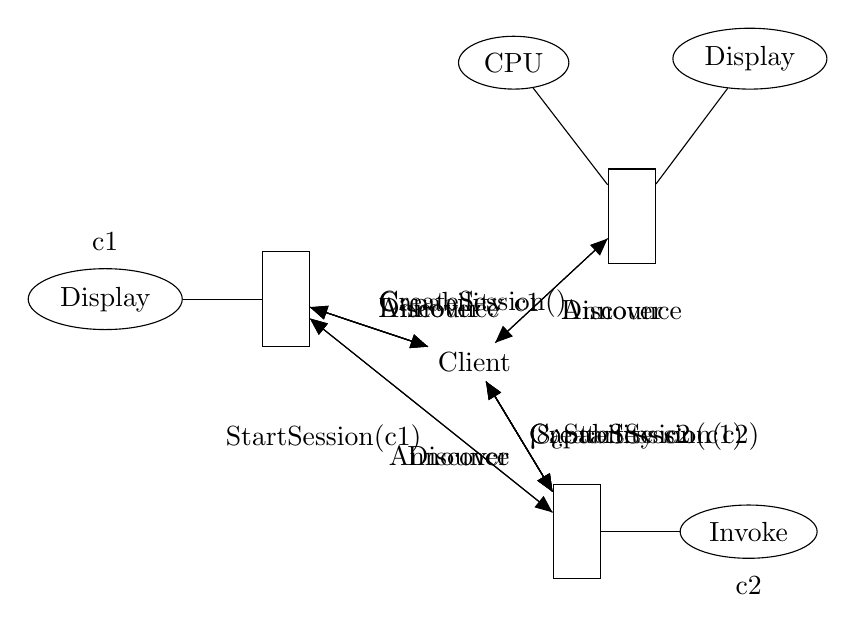
\begin{tikzpicture}[
                bidi/.style={draw, triangle 45-triangle 45},
                invoke/.style={draw, -triangle 45},
                server/.style={draw, rectangle, minimum height=1.2cm, minimum width=0.6cm},
                service/.style={draw, ellipse}
            ]

            \node (client) {Client};

            \visible<2->{
                \node[server, left=1.5cm of client,  yshift=0.8cm] (s1) {};
                \node[server, above=1.0cm of client, xshift=2.0cm] (s2) {};
                \node[server, below=1.3cm of client, xshift=1.3cm] (s3) {};
            }

            % Discover
            \visible<2>{
                \path[invoke] (client) to node[above right] {Discover} (s1);
                \path[invoke] (client) to node[below right] {Discover} (s2);
                \path[invoke] (client) to node[below left] {Discover} (s3);
            }

            % Announce
            \visible<3>{
                \path[invoke] (s1) to node[above right] {Announce} (client);
                \path[invoke] (s2) to node[below right] {Announce} (client);
                \path[invoke] (s3) to node[below left] {Announce} (client);
            }

            % Services
            \visible<3->{
                \node[service, left=of s1] (display) {Display};
                \path[draw] (display) -- (s1);

                \node[service, above=of s2, xshift=-1.5cm] (cpu2) {CPU};
                \node[service, above=of s2, xshift=+1.5cm] (display2) {Display};
                \path[draw] (cpu2) -- (s2);
                \path[draw] (display2) -- (s2);

                \node[service, right=of s3] (invoke) {Invoke};
                \path[draw] (invoke) -- (s3);
            }

            % CreateSession
            \visible<4>{
                \path[invoke] (client) to node[above right] {CreateSession()} (s1);
            }
            \visible<5>{
                \path[invoke] (s1) to node[above right] {Capability c1} (client);
            }
            \visible<5-10>{
                \node[above=1mm of display] {c1};
            }

            % CreateSession
            \visible<6>{
                \path[invoke] (client) to node[right] {CreateSession(c1)} (s3);
            }
            \visible<7>{
                \path[invoke] (s3) to node[right] {Capability c2} (client);
            }
            \visible<7-8>{
                \node[below=1mm of invoke] {c2};
            }

            % StartSession
            \visible<8>{
                \path[invoke] (client) to node[right] {\only<8>{StartSession(c2)}} (s3);
            }
            \visible<9->{
                \path[bidi] (client) to node[right] {} (s3);
            }

            % StartSession
            \visible<10>{
                \path[invoke] (s3) to node[below left] {StartSession(c1)} (s1);
            }
            \visible<11->{
                \path[bidi] (s3) to node[below left] {} (s1);
            }
        \end{tikzpicture}
    \end{figure}
\end{frame}

\begin{frame}{Protocol - Low Level}
    \begin{figure}
    \centering

    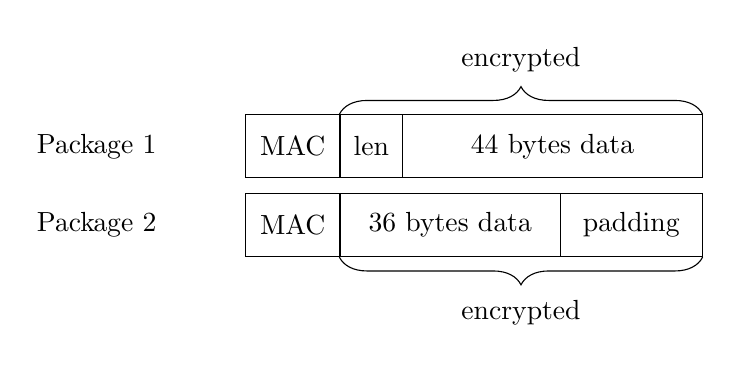
\begin{tikzpicture}[
            every node/.style={ minimum width=6mm, minimum height=8mm },
            start chain=1 going right,
            start chain=2 going right,
            node distance=-0.15mm
        ]

        \node[draw, on chain=1, minimum width=12mm] {MAC};
        \node[draw, on chain=1, minimum width=8mm ] {len};
        \node[draw, on chain=1, minimum width=38mm] {44 bytes data};
        \node[left=1cm of 1-1] {Package 1};

        \node[draw, on chain=2, minimum width=12mm, below=1cm of 1-1.west, anchor = west] {MAC};
        \node[draw, on chain=2, minimum width=28mm] {36 bytes data};
        \node[draw, on chain=2, minimum width=18mm] {padding};
        \node[left=1cm of 2-1] {Package 2};

        \draw [decorate,decoration={brace,amplitude=10pt}] (1-2.north west) -- (1-3.north east) node[midway,yshift=7mm] {encrypted};
        \draw [decorate,decoration={brace,amplitude=10pt,mirror}] (2-2.south west) -- (2-3.south east) node[midway,yshift=-7mm] {encrypted};
    \end{tikzpicture}
    \end{figure}
\end{frame}

\begin{frame}[fragile]{Protocol - Connection Establishment}
    \begin{figure}
        \centering

    \resizebox{!}{\textheight}
    {
    \begin{sequencediagram}
        \newthread{c}{Client $C$}
        \newinst[7]{s}{Service $S$}

        \begin{call}{c}{GenerateSid()}{c}{$sid$}
        \end{call}

        \postlevel

        \begin{call}{c}{GenerateKeypair()}{c}{($enc_C$, $dec_C$)}
        \end{call}

        \postlevel

        \begin{messcall}{c}{$C$, $sid$, $enc_c$}{s}

        \begin{call}{s}{GenerateKeypair()}{s}{($enc_S$, $dec_S$)}
        \end{call}

        \begin{messcall}{s}{$S$, $sid$, $enc_s$, Sign$(S, S \mathbin{\|} sid \mathbin{\|} enc_s \mathbin{\|} enc_c \mathbin{\|} C)$}{c}
        \end{messcall}

        \begin{messcall}{c}{$C$, $sid$, Sign$(C, C \mathbin{\$} sid \mathbin{\|} enc_c \mathbin{\|} enc_s \mathbin{\|} S)$}{s}
        \end{messcall}

        \begin{call}{c}{CalculateKey($enc_S$, $dec_C$)}{c}{Key}
        \end{call}

        \prelevel
        \prelevel

        \begin{call}{s}{CalculateKey($enc_C$, $dec_S$)}{s}{Key}
        \end{call}

        \end{messcall}
    \end{sequencediagram}
    }
    \end{figure}
\end{frame}

\begin{frame}{Protocol - Discovery}
    \begin{columns}[t]
        \begin{column}{0.44\textwidth}
            \lstinputlisting[caption=Probe,firstline=16]{resources/proto/discovery.proto}
        \end{column}
        \begin{column}{0.44\textwidth}
            \lstinputlisting[caption=Answer,firstline=3,lastline=14]{resources/proto/discovery.proto}
        \end{column}
    \end{columns}
\end{frame}

\begin{frame}{Protocol - Query}
    \begin{columns}[t]
        \begin{column}{0.44\textwidth}
        \end{column}
        \begin{column}{0.44\textwidth}
            \lstinputlisting[caption=Answer,firstline=14,lastline=21]{resources/proto/connect.proto}
        \end{column}
    \end{columns}
\end{frame}

\begin{frame}{Protocol - Session Estalibshment}
    \begin{columns}[t]
        \begin{column}{0.48\textwidth}
            \lstinputlisting[caption=Request,firstline=29,lastline=32]{resources/proto/connect.proto}
        \end{column}
        \begin{column}{0.40\textwidth}
            \lstinputlisting[caption=Answer,firstline=34,lastline=38]{resources/proto/connect.proto}
        \end{column}
    \end{columns}
\end{frame}

\begin{frame}{Protocol - Session Initiation}
    \begin{columns}[t]
        \begin{column}{0.44\textwidth}
            \lstinputlisting[caption=Request,firstline=39,lastline=41]{resources/proto/connect.proto}
        \end{column}
        \begin{column}{0.44\textwidth}
            \lstinputlisting[caption=answer,firstline=47,lastline=49]{resources/proto/connect.proto}
        \end{column}
    \end{columns}
\end{frame}

\begin{frame}{Service - Invoke}

    \begin{figure}
        \centering

        \resizebox{0.8\textwidth}{!}
        {
            \begin{sequencediagram}
                \newthread{c}{Client}
                \newinst[4]{s}{Service}
                \newinst[4]{i}{Invoker}

                \begin{call}{c}{Initiate(Parameters)}{s}{Service Session}
                    \begin{call}{s}{CreateSession()}{s}{Capability}
                    \end{call}
                \end{call}

                \postlevel

                \begin{call}{c}{Initiate(ServiceSession)}{i}{Invoker Session}
                    \begin{call}{i}{CreateSession()}{i}{Capability}
                    \end{call}
                \end{call}
                \postlevel

                \begin{messcall}{c}{Start}{i}
                    \begin{messcall}{i}{Start}{s}
                        \postlevel
                    \end{messcall}
                    \prelevel
                \end{messcall}
                \prelevel
            \end{sequencediagram}
        }
    \end{figure}
\end{frame}

\begin{frame}{Service - Capabilities}
    \begin{figure}
        \centering

        \resizebox{0.8\textwidth}{!}
        {
            \begin{sequencediagram}
                \newthread{r}{Requester r}
                \newinst[2]{e}{Entity e}
                \newinst[2]{s}{Service s}
                \newinst[2]{c}{Capability Service}

                \mess{e}{Register}{c}
                \postlevel

                \begin{call}{r}{Request(e, s, params)}{c}{Capability}
                    \postlevel
                    \begin{call}{c}{Ask(r, s, params)}{e}{Capability}
                        \postlevel
                        \begin{call}{e}{Initiate(params)}{s}{Capability}
                        \end{call}
                        \postlevel
                    \end{call}
                    \postlevel
                \end{call}

                \postlevel

                \begin{messcall}{r}{Start}{s}
                    \postlevel
                \end{messcall}

                \prelevel
            \end{sequencediagram}
        }
    \end{figure}
\end{frame}

\begin{frame}{Current state}
    \begin{columns}
        \begin{column}{0.40\textwidth}
            \begin{itemize}
                \item builds on
                    \begin{itemize}
                        \item Windows
                        \item Linux
                        \item OS X
                    \end{itemize}
                \item CI via Travis, Appveyor
                \item five services implemented
                    \begin{itemize}
                        \item Xpra
                        \item Input
                        \item Shell
                        \item Capabilities
                        \item Invoke
                    \end{itemize}
            \end{itemize}
        \end{column}
        \begin{column}{0.48\textwidth}
            \begin{table}
                \centering
                \begin{tabular}{c|c|c}
                    Component & LOC  & Test Cov\\
                    \hline
                    Core      & 2623 & $75\%$\\
                    Services  & 1132 & $7.3\%$\\
                    Exes      & 1301 & $0\%$\\
                    Tests     & 2361 & $100\%$\\
                    \hline
                    Total     & 8165 & $58.5\%$\\
                    &&\\
                    App       & 3409 & $0\%$
                \end{tabular}
            \end{table}
        \end{column}
    \end{columns}
\end{frame}

\begin{frame}{Related Work}
    \begin{itemize}
        \item Session establishment
            \begin{itemize}
                \item OpenSSL
                \item Diffie-Helmann
                \item libsodium/NaCl
            \end{itemize}
        \item Ticketing/capability systems
            \begin{itemize}
                \item Kerberos
                \item Plan9
                \item Eros
                \item CAP
            \end{itemize}
        \item Service implementations
            \begin{itemize}
                \item inetd/xinetd
                \item OpenSSH
            \end{itemize}
        \item Device discovery
            \begin{itemize}
                \item CryptID
                \item mDNS
                \item Matchmaking systems
            \end{itemize}
    \end{itemize}
\end{frame}

\end{document}
